\newcommand{\texCommand}[1]{\texttt{\textbackslash{#1}}}%

\newcommand{\exemplo}[1]{%
\vspace{\baselineskip}%
\noindent\fbox{\begin{minipage}{\textwidth}#1\end{minipage}}%
\\\vspace{\baselineskip}}%

\newcommand{\exemploVerbatim}[1]{%
\vspace{\baselineskip}%
\noindent\fbox{\begin{minipage}{\textwidth}%
#1\end{minipage}}%
\\\vspace{\baselineskip}}%

%%%%%%%%%%%%%%%%%%%%%%%%%%%%%%%%%%%%%%%%%%%%%%%%%%%%%%%%%%%%%%%%%%%%%%%%%%%%%%%%
%%%%%%%%%%%%%%%%%%%%%%%%%%%%%%%%%%%%%%%%%%%%%%%%%%%%%%%%%%%%%%%%%%%%%%%%%%%%%%%%
%%%%%%%%%%%%%%%%%%%%%%%%%%%%%%%%%%%%%%%%%%%%%%%%%%%%%%%%%%%%%%%%%%%%%%%%%%%%%%%%
A necessidade de mecanizar tarefas humanas data desde o período clássico da
civilização, em cerca de 350 a.C. na Grécia Antiga. Aristóteles, filosofo e
aluno de Platão, entre diversos escritos que produziu, investigou o homem, a
mente e a razão \cite{russell2004history}. Em seu livro \textit{Politiká}, um
trabalho de ética e filosofia política, Aristóteles descreve a necessidade de
automatizar tarefas humanas por meio de mecanismo que obedeçam ``palavras de
comando ou antecipação inteligente'' também chamados de ``tripods''
\cite{2013aristotle}, como forma de resolver problemas sociais, como a
escravidão. Não apenas neste trabalho, mas muito outros trabalhos foram
idealizadores do que futuramente se tornaria o campo de inteligência artificial
\cite{russell2016artificial}.

Embora a idealização de mecanizar tarefas tenha surgido na Grécia, uma
abordagem prática para isso já havia sido produzida muitos anos antes, em cerca
de 2500 a.C. Matemáticos babilônios com o objetivo de dividir grãos em
quantidades justas entre seus pares, desenvolvem uma série de etapas e
operações ordenadas para se seguir que ao final lhes garantiria o resultado
almejado \cite{chabert1999history}, esse foi um dos primeiros registros de um
conceito que hoje é nomeado `algoritmo'.

Com o advento da computação e a concepção da máquina universal, o termo
algoritmo foi adotado por esta ciência para designar instruções finitas e bem
definidas que podem ser implementadas em um computador para resolver classes de
problemas \cite{britannica2006algorithm}, o computador moderno tendo posse
então dessas ``palavras de comando'' irá então executar de forma autônoma até o
fim de sua execução, muito similar aos ``tripods'' idealizados por Aristóteles.

Porém, uma simples lista de comandos não seria suficiente para que esses
mecanismos autônomos conseguissem replicar a atuação humana em ambientes
desconhecidos, complexos e imprevisíveis \cite{russell2016artificial}, uma
parte fundamental da capacidade humana que permite lidar com essas lacunas é a
inteligência. Até o presente momento, não há um consenso sobre o que é ser
inteligente e muito menos o que é necessário para construir uma entidade
inteligente \cite{russell2016artificial}. Um grupo de 52 especialistas listou o
uso de ferramentas da mente como: perceber, memorizar, aprender, compreender,
imaginar, planejar e raciocinar \cite{gottfredson1997mainstream}, porém nossa
compreensão objetiva dessas ferramentas se aplica apenas a algumas, dentre elas
a que tivemos grande sucesso em simular foi o raciocínio
\cite{russell2016artificial}.

A principal divisão entre os tipos de raciocínio são duas, o método dedutivo e
o método indutivo. Matemáticos, lógicos e cientistas da computação com grande
sucesso tem conseguido desenvolver sistemas baseados no raciocínio dedutivo e
operar sobre premissas através e regras lógicas para provas ou verificar
teoremas, um exemplo disso são as linguagens \textit{Coq} e \textit{PROLOG}.
Aliado a isso, algoritmos de busca permitem deduzir soluções pela verificação
da árvore de eventos.

Porém o método indutivo apresenta limitações quanto a sua capacidade de
descobertas. Como demonstrado por Hume \cite{hume2000enquiry} e Kant
\cite{smith2011immanuel} certos conhecimentos não podem ser obtidos
exclusivamente através da dedução, sendo sua obtenção apenas possível pela
experimentação e percepão \cite{popper2005logic}, logo máquinas que pretendam
simular o raciocínio humano devem ter a capacidade de generalizar regras gerais
a partir de eventos singulares.

% Presente em diversos organismos na natureza \cite{shettleworth2001animal}, a
% aprendizagem é uma das ferramentas cognitivas que permite não necessitar de
% informações completas e permite lidar com incerteza gerando soluções quase
% ótimas aos problemas. Um exemplo do processo de aprendizado é observado em
% ratos evitando iscas envenenadas. Num primeiro momento em que ratos encontram
% comidas com aspectos ou cheiros desconhecidos, eles inicialmente irão comer
% apenas pequenas quantidades, e dependendo do resultado dessa experiência, caso
% a comida produza más sensações, a comida será associada a algo ruim e
% subsequentemente será evitada, o processo chamado ``aversão condicionada ao
% sabor'' \cite{garcia1955conditioned}.

% Tal motivações criaram a terceira abordagem para máquinas operarem tarefas
% humanas, o Aprendizado de Máquina, essa que se mostrou bem sucedida em tarefas
% que as outras abordagens não apresentavam desempenho tolerável.
Na próxima seção definimos o aprendizado em seu aspecto computacional,
diferente do aprendizado estatístico como em \cite{friedman2001elements}, este
trabalho será baseado nas teorias computacionais de aprendizado
\cite{valiant1984theory,gold1967language,kearns1994introduction} evidenciando
as limitações de computabilidade.

\section{Aprendizado de Máquina}
\label{sec:aprendizado-de-maquina}

No contexto de inteligência artificial, o \textbf{Aprendizado}, ou Aprendizado
de Máquina (AM), é o estudo e a concepção de agentes que melhoram o seu
desempenho nas tarefas futuras após fazer observações sobre o mundo
\cite{russell2016artificial, mohri2018foundations}. Em
\cite{mitchell1997machine} é formalmente definido como:

\begin{definition}
Um programa de computador (agente), \textit{aprende} de uma experiência
$\boldsymbol E$ a respeito de alguma classe de tarefa $\boldsymbol T$ e medida
de performance $\boldsymbol P$, se a performance na tarefa $\boldsymbol T$,
medido por $\boldsymbol P$, melhora com a experiência $\boldsymbol E$.
\end{definition}

No modelo \textbf{supervisionado}\footnote{A literatura subdivide problemas de
aprendizado em supervisionado, não supervisionado e por reforço
\cite{russell2016artificial,friedman2001elements,goodfellow2016deep},
porém há outros paradigmas mais gerais, como a identificação de linguagem no
limite \cite{gold1967language}}, o qual lidaremos exclusivamente neste
trabalho, a experiência $\boldsymbol E$ é um registro
$\boldsymbol{x}=(x_1,x_2,...,x_n)$, em que $x_i$ é um valor real computável
($\mathbb{R}_c$), e seu respectivo rotulo $y$. A tarefa $\boldsymbol T$
consiste em atribuir um valor $\hat{y}$ para um $\boldsymbol{x}$ onde o $y$
real ainda não é conhecido, mas assumindo que esse par ordenado
$(\boldsymbol{x},y)$ será gerado por um programa desconhecido porém que
assumimos sua invariância e regularidade de aprendizagem
\cite{mohri2018foundations,valiant1984theory}.

Para isto, queremos induzir através dos pares de experiência
($\boldsymbol{x},y$) uma \textbf{função computável} $f_c$, isto é, uma máquina
de Turing (MT) que sobre a entrada $\boldsymbol{w}$ para com exatamente
$f_c(\boldsymbol{w})$ sobre sua fita, de tal forma que ao mensurarmos
observações futuras de $f_c(\boldsymbol{x})$ por $\boldsymbol P$, o valor de
$\boldsymbol{P}(\hat{y},y)$ tenda a um erro irredutível
\cite{mohri2018foundations,mitchell1997machine,friedman2001elements}.

Codificaremos $y$ em dois tipos de tarefas em $\boldsymbol{T}$, na primeira
queremos computar uma cadeia de bits que representa um valor \textbf{real
computável} a partir da entrada $\boldsymbol{x}$, ou seja, queremos uma $f_c$
tal que $f_c:\mathbb{R}_c^n\longrightarrow \mathbb{R}_c$, essa tarefa
denominamos \textbf{regressão}. Na segunda tarefa, queremos descobrir a função
$f$ que tenha como saída um único bit, de tal forma que
$f:\mathbb{R}_c^n\longrightarrow \{0,1\}$, essa tarefa denominamos
\textbf{classificação}\footnote{Embora definido para duas classes o formalismo
descrito aqui pode ser estendido para mais de duas classes com métodos
multi classe \cite{abu2012learning}.} \cite{goodfellow2016deep,
mohri2018foundations}.

O processo indutivo descrito anteriormente aparenta ser uma tarefa fácil, porém
para um número finitos de exemplos existem infinitas funções ($f_c$) que
interpolam perfeitamente todos esses
pontos\cite{bishop2006pattern,abu2012learning}, entretanto, para que se tenha
um bom desempenho em tarefas futuras, tal função deve se aproximar do real
programa gerador dos dados
\cite{mohri2018foundations,goodfellow2016deep,solomonoff1964formal,kearns1994introduction},
o que nos leva a pergunta: ``qual dessas funções deve ser escolhida?''

Um princípio que pode ser adotado nessa escolha, é o chamado \textit{"Navalha
de Ockham"} \cite{blumer1987occam}, ele diz que para duas hipóteses de igual
poder explicativo, é preferível escolher a \textit{mais simples}. No inicio do
desenvolvimento de técnicas de inferência indutiva, não havia uma definição
formal do que seria uma hipótese ``mais simples'', em 1964 com o trabalho de
Solomonoff da teoria de inferência indutiva universal
\cite{solomonoff1964formal}, é apresentada uma definição formal para o que
seria esse principio: a MT de menor comprimento que computa tal observação,
isso é, a $f_c$ com menor complexidade de Kolmogorov. Esse sistema indutivo do
ponto de vista teórico pode ser considerado perfeito \cite{li1992inductive}, já
que assumindo que o mundo é gerado por um programa desconhecido, na
distribuição de probabilidade algorítmica, programas de menor descrição são os
mais prováveis.

Porém já se sabe que tal MT (programa) é \textbf{indecidível}, pois escolher um
programa equivalente de menor comprimento é mapeável ao problema da parada
\cite{sipser2012introduction,solomonoff1978complexity}, logo, no caso geral,
seria impossível descrever um \textbf{método efetivo} para proceder tal escolha
\cite{hutter2004universal}. Uma solução a esse problema\footnote{As teorias
Dimensão VC \cite{vapnik2013nature}, Complexidade de Rademacher
\cite{bartlett2002rademacher} e PAC \cite{valiant1984theory} são casos
restritos da inferência indutiva universal
\cite{li1992inductive,blumer1989learnability}} é definir \textit{a priori} um
espaço de hipóteses $\mathcal{H}$ (programas) de menor
cardinalidade\footnote{Também referido como Viés.}, e.g. todos os programas que
podem ser descritos em Python com no máximo $10^9$ bits, assim, algoritmos
efetivos poderiam escolher os programas de menor descrição em seu respectivo
$\mathcal{H}$ \cite{rathmanner2011philosophical}.

Embora não exista uma máquina de Turing (MT) que resolva o caso geral, a teoria
Provavelmente Aproximadamente Correto de aprendizado nos dá a garantias da
existência de máquinas que resolvam em tempo polinomial, isto é, para alguma
amostra de tamanho $n$, existe uma MT que com tempo $O(n^k)$ para algum $k \in
\mathbb{N}$, encontra uma MT $c$ que mapeia
$c:\mathcal{X}\rightarrow\mathcal{Y}$, de tal forma que essa MT se aproxime da
real função geradora $f_c$ com alta probabilidade. Para isso a classe de
programas geradores que se pode assumir deve ser limitada, apenas dados gerados
de forma independente por uma distribuição estacionaria nos garante a validade
das propriedades dos teoremas apresentados a seguir.

Limitamos as funções computáveis que queremos descobrir a retângulos que
classificam pontos em $\mathbb{R}^2$ , os quais pertencem aos conjunto de
conceitos $\mathcal{C}$. Seja um retângulo $c$ de tal forma que $c$ classifique
o ponto em 1 se contido dentro do retângulo ou 0 c.c, isto é,
$c:\mathcal{X}\rightarrow\mathcal{Y}$, sendo $\mathcal{X} \in \mathbb{R}^2$, as
coordenadas no plano cartesiano e $\mathcal{Y} \in \{0,1\}$, a classe ao qual
aquele ponto é atribuída. O algoritmo deve conter um espaço de hipóteses fixo
$\mathcal{H}$ que não necessariamente coincida com $\mathcal{C}$ e obter
amostras $S=(X_1,X_2,...,X_m)$ obtidas da distribuição $\mathcal{D}$, esta
i.i.d. (independente e identicamente distribuído) como descrito anteriormente.

\textcolor{red}{falar do pac learning, np-complexidade}

Existe uma diversidade de algoritmos para seleção de hipóteses
\cite{bishop2006pattern,friedman2001elements}, neste trabalho apresentaremos a
Árvore de Decisão, e algoritmos derivados como Floresta Aleatória e Máquinas de
Reforço (\textit{Boosting}) do Gradiente, também apresentaremos as Máquinas de
Vetores de Suporte.

\subsection{Árvores de Decisão}
Árvores de Decisão são modelos que devido sua simplicidade tem fácil
interpretabilidade e podem ser combinado com técnicas de amostragem e reforço
em algoritmos em modelos muito mais poderosos. Embora exista um diversidade de
algoritmos para sua concepção nos basearemos no modelo CART proposto em
\cite{breiman1984classification}, a intuição por trás desse algoritmo é
particionar o espaço de atributos $\mathcal{X}$ em regiões em $R_i$, de
tal forma que cada $R_i$ se aproxime do valor médio de $\mathcal{Y}$ para
aquela região.

\begin{figure}[ht]
   \centering
    \begin{subfigure}{.4\textwidth}
        \centering
        \def\svgwidth{1.4\linewidth}
        \incfig{binarytree}
        \caption{Árvore de decisão com predicados booleanos sobre os atributos.}
        \label{fig:tree}
    \end{subfigure}
     \hfill
    \begin{subfigure}{.4\textwidth}
        \centering
        \def\svgwidth{.8\linewidth}
        \incfig{splitregion}
        \caption{Plano cartesiano particionado por uma árvore de decisão.}
        \label{fig:split}
    \end{subfigure}
    \caption{Exemplo de árvore de decisão}
    \label{fig:three graphs}
\end{figure}


Na Figura \ref{fig:split} é exemplificado um particionamento dado pela árvore
da Figura \ref{fig:tree}, na raiz da árvore de decisão é aplicado um predicado
booleano que irá dividir os dados em dois subconjuntos, a cada divisão nos nós
esses subconjuntos são aplicados a novos predicados gerando subconjuntos
menores.

Explicada o funcionamento das árvores, detalhamos agora como construí-las. Para
isso, é feito uma busca exaustiva em todos os atributos $j$ e seus valores
$t_m$ bi particionando os dados em $\theta = (j,t_m)$ como mostrado em
\ref{eq:splitc}.

\begin{equation}
        \begin{aligned}
            Q_{\text{left}}(\theta) = {(x, y) | x_j <= t_m}\\
            Q_{\text{right}}(\theta) = Q \setminus Q_{\text{left}}(\theta)
        \end{aligned}
    \label{eq:splitc}
\end{equation}

De tal forma a minimizar $L$ sobre a função de
impureza $H$.

\begin{equation}
    \underset{\theta}{\text{arg min}} \left[ L(\theta) =  \frac{n_{\text{left}}}{N_m} H(Q_{\text{left}}(\theta)) +
    \frac{n_{\text{right}}}{N_m} H(Q_{\text{right}}(\theta)) \right]
    \label{eq:treegreed}
\end{equation}

Para o calculo do $H$ é dado pela proporção de classes na região $R_m$,
dado $N_m$ observações, em razão do erro de classificação.

\begin{equation}
    p_{mk} = \frac{1}{N_m} \sum_{x_i \in R_m} I(y_i = k)
\end{equation}

Em \cite{friedman2001elements} são apresentados alguns dos critérios que podem
ser usados para computar a impureza da classificação, aqui aplicaremos o índice
Gini.

\begin{equation}
    H(X_m) = \sum_{k=1}^{K} \hat{p}_{mk}(1 - \hat{p}_{mk})
    \label{eq:gini}
\end{equation}

Esse particionamento é então aplicado recursivamente até que seja atingido
algum critério de regularização, por exemplo, o limite mínimo para $m$ ou
definido um valor minimo para $H$.

Embora árvores de decisão tenha diversas vantagens, elas tendem a sobreajustar
aos dados, uma possível solução para isso é o uso de comitês.

\subsection{Floresta Aleatória}

Árvores de decisão podem ``decorar'' os dados de treino, não generalizando para
casos desconhecidos, o chamado sobreajuste. O \textit{Bagging}, uma técnica de
reamostragem, tenta diminuir esse sobreajuste por meio da diminuição da
variação entre os modelos, ou seja, modelos obtidos de forma independente
tendam a uma mesma predição. Ele consiste em designar subamostras aleatórias
(com repetição) do conjunto de dados e ao final as estimativas desses modelos
são combinadas.

Porém ainda assim, dado a natureza determinística e a flexibilidade de uma
árvore de decisão o problema do sobreajuste pode não ser resolvido, é
necessário então aleatorizar o processo de geração da árvore. O método de
subespaço aleatório (\textit{random subspace method}) provê isso limitando o
espaço de busca por bipartições da árvore, a cada novo nó da árvore que está
sendo construída, apenas um subconjunto aleatório dos atributos pode ser
escolhido para a bipartição dos dados.

\begin{algorithm}[ht]
\SetKwInput{KwInput}{Input}
\SetKwInput{KwOutput}{Output}
\KwData{Conjunto de dados $D$ com atributos $p$.}
\KwInput{$B$ - Número de estimadores a serem construídos, $m$ - Número de atributos
nos subconjuntos.}
\KwOutput{Classificador - Maioria dos votos de $\{T_b\}^B$.}
\begin{enumerate}
    \item Para $b=1$ até $B$.
    \begin{enumerate}
        \item Obtenha um subconjunto aleatório com repetição
            (\textit{Bootstrap}) de $D$.
        \item Construa uma árvore $T_b$ recursivamente da seguinte forma:
        \begin{enumerate}
            \item Selecione m variáveis do conjunto $p$.
            \item Selecione a melhor variável e bipartição em $m$.
            \item Divida o nó em dois nós filhos.
        \end{enumerate}
    \end{enumerate}
    \item Retorne o conjunto de arvores $\{T_b\}^B$.
\end{enumerate}
 \caption{Floresta Aleatória}
 \label{algo:rf}
\end{algorithm}

Essa limitação garante que as árvores de entropia máxima não possam ser sempre
geradas, diminuindo a correlação entre as árvores e, portanto, melhorando a
capacidade de generalização desse estimador. No Algoritmo \ref{algo:rf} é
apresentado o pseudo-código da Floresta Aleatória.

\subsection{Máquina de Reforço do Gradiente}

O algoritmo de Floresta Aleatória nos dá uma ideia do poder que temos ao
combinar algoritmos simples, também chamado \textit{weak learner}, em
algoritmos mais robustos. Uma outra alternativa a combinação de modelos é o
Reforço, ou \textit{Boosting}, esse consiste em criar estimadores a partir do
resíduo de estimadores anteriores, assim esse novo estimador tem uma tarefa
mais simples e logo, quando combinado com toda a sequência de estimadores, pode
apresentar maior robustez no aprendizado.

Demonstramos anteriormente como árvores CART são induzidas, sendo $R_j,j=1,2,..J$ as regiões particionadas pela árvore, se $x \in R_j \implies f(x) = \gamma_j$, que no caso de classificação $\gamma_j$ é o valor modal daquela região. Logo podemos definir formalmente como

\begin{equation}
    T(x;\Theta) = \sum_{j=1}^J \gamma_j I(x \in R_j),
\end{equation}

sendo $\Theta = \{R_j,\gamma_j\}_1^J$ parâmetros obtidos minimizando o risco empírico dado por

\begin{equation}
    \hat{\Theta} = \underset{\Theta}{\text{arg min}}
    \sum_{i=1}^N L(y_i,T(x;\Theta)).
\end{equation}

Logo, as árvores de reforço são dadas por

\begin{equation}
\label{eq:tree_boost}
    f_M(x) = \sum_{m=1}^M T(x;\Theta_m),
\end{equation}

induzidas sequencialmente resolvendo

\begin{equation}
    \hat{\Theta}_m = \underset{\Theta_m}{\text{arg min}}
    \sum_{i=1}^N L(y_i,f_{m-1}(x_i)+T(x_i;\Theta_m)),
\end{equation}

logo, cada árvore deve aprender apenas o resíduo do erro da árvore anterior, isto é, a árvore $m$ deve predizer $y_i - f_{m-1}(x_i)$. Porém o método descrito aqui embora seja intuitivo e correto, é ineficiente, sendo preferível sua aproximação que pode ser obtida em um único passo e não sequencialmente.

Definimos a função de custo por

\begin{equation}
    L(f) = \sum_{i=1}^N L(y_i,f(x_i)),
\end{equation}

portanto, queremos minimizar $L(f)$ em função de $f$, onde $f$ é descrita na equação \ref{eq:tree_boost}. Logo, sendo $\boldsymbol{f}$ as funções que aproximam $f(x_i)$ em cada ponto $x_i$ de $N$, fazemos
\begin{equation}
\label{eq:step_boost}
\hat{\boldsymbol{f}} = \underset{\boldsymbol{f}}{\text{arg min }}L(\boldsymbol{f}).
\end{equation}

Usamos então o método do gradiente para otimizar a equação \ref{eq:step_boost}, sendo $\rho$ a taxa de aprendizado atualizamos
\begin{equation}
    \boldsymbol{f}_m = \boldsymbol{f}_{m-1} - \rho_m \boldsymbol{g}_m,
\end{equation}
onde os componentes do gradiente $\boldsymbol{g}_m$ são dados por
\begin{equation}
    g_{im} = \left[ \frac{\partial L(y_i,f(x_i))}{\partial
                f(x_i)} \right]_{f(x_i)=f_{m-1}(x_i)}.
\end{equation}

A implementação detalhada deste algoritmo está apresentada pelo pseudo-código do Algoritmo \ref{algo:gbm}.

\begin{algorithm}[ht]
    \SetKwInput{KwInput}{Input}
    \SetKwInput{KwOutput}{Output}
    \KwData{Conjunto de dados D com atributos p.}
    \KwInput{M - Número de estimadores a serem construídos.}
    \KwOutput{Classificador - $f_M(x)$.}
    \begin{enumerate}
        \item Construa $f_0(x) = \textit{arg min}_\gamma \sum_{i=1}^N$
        \item Para $m=1$ até $M$.
        \begin{enumerate}
            \item Para $i=1,2,..,N$ calcule
                \[ r_{im} = - \left[ \frac{\partial L(y_i,f(x_i))}{\partial
                f(x_i)} \right]_{f=f_{m-1}}\]
            \item obtenha a árvore de regressão para os $r_{im}$ dada as
                regiões terminais $R_{jm}, j=1,2,..,J_m$.
            \item Para $j=1,2,..,J_m$ calcule
                \[\gamma_{jm} = \sum_{x_i \in R_{jm}}
                L(y_i,f_{m-1}(x_i)+\gamma)\]
            \item Atualize $f_m(x) = f_{m-1}(x) +
                \sum_{j=1}^{J_m} \gamma_{jm}I(x \in R_{jm})$.
        \end{enumerate}
        \item Retorne $\hat{f}(x) = f_M(x)$.
    \end{enumerate}
    \caption{Máquina de Reforço do Gradiente}
    \label{algo:gbm}
\end{algorithm}


\subsection{Máquina de Vetores de Suporte}
Máquinas de vetores de suporte são construídas em cima de duas idéias muito
elegantes do ponto de vista teórico, classificadores de máxima margem e
projeções vetoriais. Classificadores de máxima margem obtém um hiperplano de
solução unica tal que a margem entre esse hiperplano e os pontos de duas
classes, se linearmente separáveis, seja máximo, resultando em um hiperplano
com garantias de uma boa generalização \cite{vapnik2013nature}.

\begin{figure}[ht]
   \centering
    \begin{subfigure}{.48\textwidth}
        \centering
        \def\svgwidth{\linewidth}
        \incfig{maxmargin}
    \end{subfigure}
     \hfill
    \begin{subfigure}{.48\textwidth}
        \centering
        \def\svgwidth{\linewidth}
        \incfig{svm}
    \end{subfigure}
    \caption{Máquina de vetores de suporte. A direita temos exemplos de dados
    que são linearmente separáveis logo é possível margens rigidas e a direita
    dados não-linearmente separáveis onde são necessárias margens permissivas.
    Os pontos $\xi_i$ são aqueles que estão do lado errado do plano.}
    \label{fig:svm}
\end{figure}

Porém, uma vasta gama problemas não apresenta uma separação linear entre as
classes, sendo necessárias duas abordagens generalizar esse algoritmo, projetar
os dados em uma dimensão em que sejam linearmente separaveis, possívelmente uma
dimensão infinita através do ``truque de núcleo'' (\textit{kernel trick}), e
também tornar as margens menos restritas para se adaptarem a ruídos nos dados.
Inicialmente definimos o hiperplano como

\begin{equation}
    \label{eq:svm_func}
    x^T\beta + \beta_0 = 0
\end{equation}

Sendo $\beta$ o vetor unitário, isto é $\Vert\beta\Vert = 1$ e a regra de
classificação é dada por

\begin{equation}
    \label{eq:svm_sign}
    G(x) = \text{sign}(x^T\beta + \beta_0)
\end{equation}

Para obter o hiperplano de máxima margem otimizamos $\beta$ restringindo o
critério de otimização de tal forma que suavize para os pontos $\xi_i$, logo

\begin{equation}
    \underset{\beta,\beta_0}{\text{min}} \frac{1}{2}\Vert\beta\Vert^2 +
    C\sum_{i=1}^{N}\xi_i \hspace{1em} \text{subject to } \xi_i \geq 0,
    y_i(x_i^T\beta+\beta_0) \geq 1-\xi_i \forall i
\end{equation}

Onde $C$ é um hiperparametro definido \textit{a priori} que ajusta a rigidez
das margens quanto a pontos erroneamente classificados. Essa operação tem por
forma primal de Lagrange

\begin{equation}
    \label{eq:lag_svm}
    L_p = \frac{1}{2}\Vert\beta\Vert^2 + C\sum_{i=1}^{N}\xi_i -
    \sum_{i=1}^{N}\alpha_i [y_i(x_i^T\beta+\beta_0) - (1-\xi_i)] -
    \sum_{i=1}^{N}\mu_i\xi_i
\end{equation}

Porém como anteriormente discutido, nem todos os problemas podem ser
linearmente separáveis, o que limitaria e muito a aplicabilidade desse
algoritmo, uma alternativa a isso é projetar os dados em uma dimensão em que as
classes sejam separáveis pelo hiperplano, essa projeção é feita por uma função
$h(x)$, for exemplo $h(x) = (x_1^2, x_2^2, x_1^2+x_2^2)$ como mostrado na
Figura \ref{fig:svm_kernel}.

\begin{figure}[ht]
   \centering
    \def\svgwidth{\linewidth}
    \incfig{svm_kernel}
    \caption{Operação de núcleo sobre os dados. A esquerda dados que não são
    linearmente separáveis se transformam em separáveis com a projeção
    demonstrada na figura a direita.}
    \label{fig:svm_kernel}
\end{figure}

Desta forma, rescrevemos a função do hiperplano \ref{eq:svm_func} como

 \begin{equation}
    \label{eq:svm_kernel}
    h(x)^T\beta + \beta_0 = 0
\end{equation}

Pela forma da equação \ref{eq:lag_svm} e \ref{eq:svm_sign} reescrevemos o
o classificador da seguinte forma

\begin{equation}
    G(x) = \text{sign}
    \left(\sum_{i=1}^N \alpha_i y_i \langle h(x),h(x_i)\rangle+\beta_0 \right)
\end{equation}

A literatura costuma apresentar tres escolhas populares para núcleo, que são

\begin{equation}
    \begin{split}
        \text{Polinomial:} &\quad (1+\langle x,x_i\rangle)\\
        \text{Base Radial:} &\quad \text{exp}(-\gamma \Vert x - x_i\Vert^2)\\
        \text{Rede Neural:} &\quad \text{tanh}(k_1\langle x,x_i\rangle+k_2)
    \end{split}
\end{equation}

Devido a elegância teórica desse algoritmo a sua generalização é dada em função
da quantidade de vetores de suporte escolhidos, e embora essa projeção aumente
a dimensionalidade dos dados, no caso do núcleo de base radial para uma
dimensão infinita, ele ainda tem garantias de ter um baixo erro fora dos dados
conhecidos \cite{vapnik2013nature}.

\subsection{``Não existe almoço grátis''}
Vimos a viabilidade e descrevemos o projeto de alguns algoritmos, surge então a
seguinte questão: ``Para um dado problema com caracteristicas $Z$, qual desses
algoritmos deve ser selecionado?''. Como apresentado pelo teorema do \textit{No
Free Lunch} em \cite{wolpert1997no,wolpert1996lack}, não há uma distinção
formal \textit{a priori} entre esses algoritmos que aponte qual é o mais
adequado a um dado problema. Logo, métodos experimentais e estatisticos são
aplicados nessa tarefa, como conjutos de validação, para comparar e selecionar
algoritmos. Porém está abordagem apresenta algumas limitações dada a
insuficiência estatistica ou viéses causados pelo método empirico.

Neste trabalho buscamos automatizar e diminuir problemas causados pela seleção
empirica de algoritmos, usando informações \textit{a posteriori} do espaço de
instâncias para essa escolha, essa abordagem também conhecida como
meta-aprendizado.

\section{Meta-Aprendizado}
\label{sec:metalearning}
O problema de seleção de algoritmos foi inicialmente observado por J. R. Rice
(1976) \cite{Rice1976} com o principal objetivo de prever o melhor algoritmo
para resolver um dado problema quando houver mais de um algoritmo que resolva
disponível.
Os componentes desse modelo são: o espaço de instâncias do problema ($P$), que
é composto por conjuntos de dados em Meta-Aprendizado (MtA); o espaço de
instâncias de atributos ($F$), que são os meta-atributos usados para descrever
os conjuntos de dados; o espaço de algoritmos ($A$), que contém um conjunto de
algoritmos de AM que podem ser recomendados; e um espaço de medidas de
avaliação ($Y$), responsável por recuperar as performances dos algoritmos de AM
que resolvem as instâncias dos problemas contidos em $P$.
Usando os conjuntos descritos anteriormente, um sistema de MtA pode criar o
mapeamento de um conjunto de dados $p$ descrimináveis pelos meta-atributos $f$
em um ou mais algoritmos $\alpha$, de tal forma que a recomendação de
algoritmos por sistema tenha uma performance medida por $y$ tolerável, e.g.,
com máximo $y(\alpha(p))$.

K. A. Smith-Miles (2008) \cite{SmithMiles2008} aprimorou esse modelo abstrato
propondo generalizações que podem também ser aplicadas ao problema do projeto
de algoritmos.  Nessa proposta, alguns componentes são adicionados: o conjunto
de algoritmos de MtA; a generalização de regras empíricas ou ranqueamento de
algoritmos; a verificação de resultados empíricos, que podem ser guiados por
uma base teórica ao aprimoramento de algoritmos.

Um componente crucial dos modelos anteriores é a definição do conjunto de
meta-atributos ($F$) usados para descrever propriedades gerais dos conjuntos de
dados. Esses meta-atributos devem ser capaz de prover evidências sobre
performance futuro dos algoritmos em $A$ \cite{Soares2001, Reif2012} e
discriminar, com baixo custo computacional, a performance de um grupo de
algoritmos. Os principais meta-atributos usados na literatura de MtA podem ser
divididos em cinco grupos: Gerais, Estatísticos, de Teoria da Informação,
Baseados em Modelo e de Landmarkings.

Os Gerais podem ser facilmente extraídos dos dados \cite{Reif2014}, com baixo
custo computacional \cite{Reif2012}.
Os meta-atributos estatísticos capturam os indicadores principais sobre
localização e distribuição dos dados, tais como média, desvio padrão,
correlação e curtose.
Meta-atributos de teoria da informação, usualmente medidas de entropia
\cite{Segrera2008}, capturam a quantidade de informação em um (sub)conjunto dos
dados \cite{SmithMiles2008}.
Já os baseados em modelo são propriedades extraídas de modelos de AM,
geralmente AD \cite{Bensusan2000, Peng2002}, induzidos dos dados sob analise
\cite{Reif2014}.
Os meta-atributos de Landmarking usam a performance de algoritmos de
aprendizado simples e rápidos para caracterizar os conjuntos de dados
\cite{SmithMiles2008}.

A definição do conjunto de instâncias de problema ($P$) é outra preocupação,
quando o ideal seria usar um grande número de conjuntos de dados diversos, com
objetivo de induzir um meta-modelo confiável.
Para reduzir o viés dessa escolha, conjuntos de dados de diversos repositórios,
tais como o UCI\footnote{\url{https://archive.ics.uci.edu/ml/index.php}}
\cite{Lichman2013} e o OpenML\footnote{\url{http://www.openml.org/}}
\cite{OpenML2013}, podem ser usados.

O espaço de algoritmos $A$ representa o conjunto de algoritmos candidatos a
serem recomendados no processo de seleção de algoritmos.
Idealmente, esses algoritmos devem também ser suficientemente distintos entre
si e representar toda a região do espaço de algoritmos \cite{Munoz2018}.
Os modelos induzidos pelo algoritmo podem ser avaliados por diferentes medidas,
para tarefas de classificação, a maioria dos estudos usando MtA usam acurácia.
Entretanto, outros indicadores, como o $F_\beta$, AUC e coeficiente Kappa,
também podem ser usados.

Após a extração dos meta-atributos dos conjuntos de dados e a mensuração da
performance do conjunto de algoritmos nesses conjuntos de dados, o próximo
passo é rotular cada meta-exemplo nos meta-dados.
Brazdil et al. (2009) \cite{Brazdil2009} resume as quatro propriedades
principais frequentemente usadas para rotular meta-exemplos em MtA: ($i$)
o algoritmo que apresenta a melhor performance no conjunto de dados (uma tarefa
de classificação); ($ii$) o ranqueamento dos algoritmos de acordo com suas
performances no conjunto de dados (uma tarefa de ranqueamento), onde o
algoritmo com melhor performance está no topo do ranque; ($iii$) o valor de
performance obtido por cada algoritmo individualmente no conjunto de dados (uma
tarefa de regressão) e; ($iv$) a descrição do modelo, que é geralmente baseado
em agrupamentos ou regras de associação.

\section{Fluxos de Dados}

\label{sec:datastreams}
Dados estáticos e bem estruturados não se apresentam como uma boa alternativa a
modelagem em ambientes com massiva interação livre de usuários, para esses
ambientes uma das possíveis abordagens são fluxos de
dados\cite{babcock2002models}.
Embora fluxos de dados sejam observados no tempo, similar a definição de uma
série temporal eles diferem de séries temporais em alguns aspectos, fluxos de
dados não tem uma frequência fixa entre as observações, sendo essa frequência
definida geralmente pela ordem aleatória da geração dos dados que pode ou não
ter uma natureza evolutiva  \cite{gama2007learning}. Outro aspecto importante
ao lidar com desse tipo de dado são as limitações de engenharia, dado que é um
conjunto infinito (não terminável) de dados e que não podem ser lidos
livremente, dado os limites computacionais impostos pela grande quantidade de
dados \cite{babcock2002models}. Por ultimo, acredita-se que fluxos de dados não
tenham dependências temporais, diferentes de séries temporais, porém em artigos
como \cite{read2018concept} é apresentado que não é isso que ocorre no caso de
mudança de conceito.

Essas limitações práticas causam limitações significativa nos métodos e
abordagens que podem ser aplicados na mineração de fluxos de dados, essa que
será tratada nessa seção. Séries temporais (e similarmente, fluxos de dados)
podem ser gerados por dois tipos de distribuições, estacionárias e
não-estacionárias, para a primeira se tem medias e variâncias constantes para
qualquer janela ao longo do tempo, já na segunda, esses dois parâmetros podem
variar em função de fenômenos conhecidos ou desconhecidos por trás do processo
gerador desses dados\cite{read2018concept}. Tais padrões de variações costumam
recorrer em diversas series por isso nomes foram atribuídos a cada
comportamento, são eles, tendência, ciclos, sazonalidade e mudança de conceito
\cite{hyndman2018forecasting,tsymbal2004problem,brockwell2016introduction}.

Tendências e ciclos geralmente descrevem eventos econômicos de crescimento (ou
decrescimento) e oscilações de subida e descida dado por flutuações de curto
prazo, para simplicidade e por esses fenômenos terem uma natureza similar, eles
são agregados em uma única componente e denominados por ``ciclo-tendência'' ou
apenas ``tendência'' \cite{hyndman2018forecasting}.

Com o passar dos anos é esperado um crescimento populacional e naturalmente a
população empregada também irá crescer, a Figura \ref{fig:trend} apresenta a
série temporal do número de pessoas formalmente empregadas nos Estados Unidos,
do ano 1947 a 1962, é observável o efeito da tendência no comportamento da
série temporal já que vemos o crescimento como descrito acima.

\begin{figure}[ht]
    \centering
    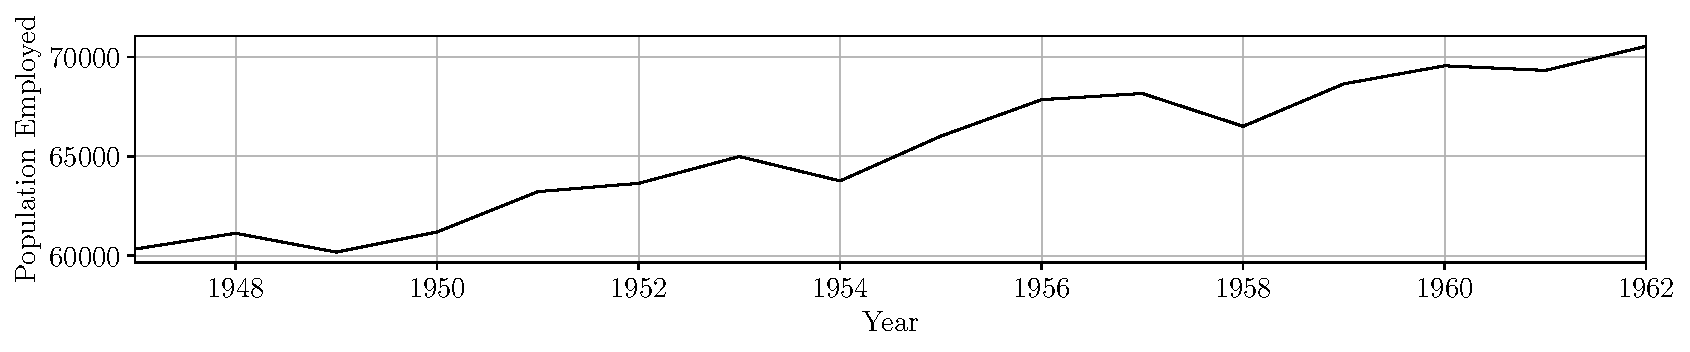
\includegraphics[width=\textwidth]{longley}
    \caption{Exemplo de tendência.}
    \label{fig:trend}
\end{figure}

Padrões sazonais ocorrem quando um fenômeno observado é afetado por fatores
sazonais, por exemplo o período do ano ou a hora do dia, esse necessariamente
de uma frequência fixa conhecida
\cite{hyndman2018forecasting,brockwell2016introduction}. Na Figura
\ref{fig:seasonality}, é apresentado uma série de observações da temperatura
média diária na cidade de Melbourne, Austrália ao longo de 10 anos, essa séria
apresenta um padrão de sazonalidade, sendo a temperatura da terra afetada pelo
ciclos solar, as estações do ano, é possível observar a periodicidade do
aumento e diminuição da temperatura relacionado a isso.

\begin{figure}[ht]
    \centering
    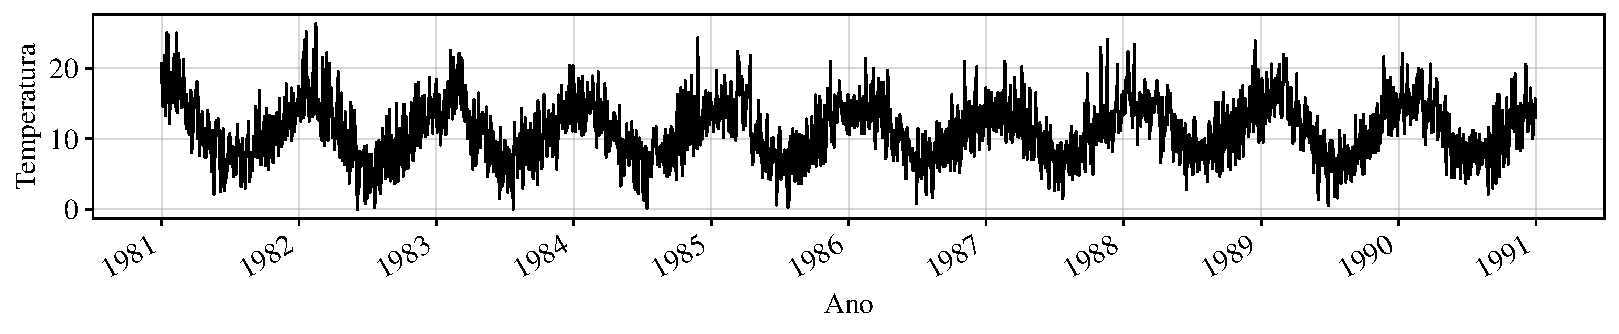
\includegraphics[width=\textwidth]{temperature}
    \caption{Exemplo de sazonalidade.}
    \label{fig:seasonality}
\end{figure}



\textcolor{red}{descrever mudança de conceito estatisticamente, detalhar}

% %http://www.dfki.de/lwa2005/fgml/paper09.pdf mudança de conceito formal nesse paper


% \begin{figure}[ht]
%     \centering
%     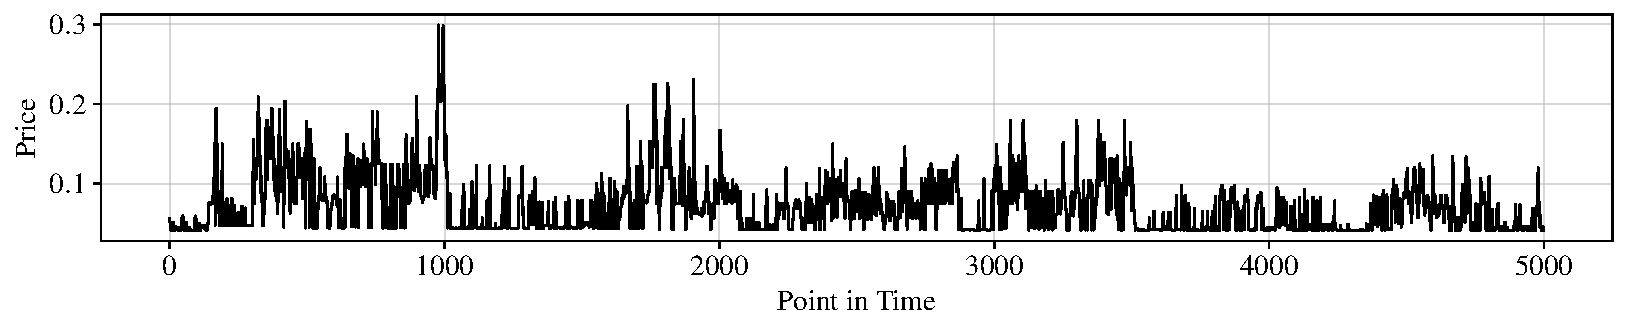
\includegraphics[width=\textwidth]{elec}
%     \caption{Exemplo de mudança de conceito.}
%     \label{fig:concept_drift}
% \end{figure}

A maioria das técnicas de AM assumem que os dados são independentes e
identicamente distribuídos (\textit{iid}), mas essas premissas geralmente não
se sustentam em ambientes de fluxos de dados, como apontado por A. Bifet and R.
Gavald\`a (2007) \cite{bifet2007learning}, dado que os dados chegam
interminavelmente e, por isso, podem apresentar dependência temporal e mudanças
de conceito pode ocorrer.  Outro aspecto critico é a imposição de limites
computacionais a esses ambientes, como memória, CPU, e largura de banda
\cite{bifet2010moa, gama2012survey}.  Para resolver esses problemas, diversas
tecnologias foram desenvolvidas. Dentre elas, as mais proeminentes são
mecanismos de esquecimento, testes estatísticos e algoritmos adaptativos.

Mecanismos de esquecimento fazem dados recentes tornarem-se mais relevantes e
dados passados menos, um exemplo são janelas deslizantes
\cite{gaber2005mining}, um método agnóstico de modelo.
Sistemas baseados em testes estatísticos agem monitorando uma métrica
pre-definida, tal como performance preditiva do modelo, e então ``disparam'' um
alarme quando a qualidade dessas métricas está abaixa de algum limiar
tolerável, demandando alguma ação.

Exemplos dessa abordagem são o teste de Page-Hinkley e o \textit{Statistical
Process Control} \cite{gama2010knowledge}.
Baseado nessas duas soluções, o \textit{ADaptive WINdowing} (ADWIN) \cite{bifet2007learning} usa testes estatísticos para definir o tamanho de cada janela, ajustando ao ``tamanho do conceito''.
Entretanto, embora esses métodos serem capazes de alarmar uma redução na performance dos modelos e adaptar o tamanho da janela a isso, não é possível identificar os algoritmos ou modelos que se tornaram mais apropriados ao novo conjunto de dados que está sendo gerado.

Algoritmos de aprendizado adaptativo, como o VFDT \cite{domingos2000mining},
foram inicialmente introduzidos com fluxos de dados em mente, desempenhando aprendizado online e baixo consumo de memoria, mas não conseguiam se adaptar a mudança de conceito, um problema já conhecido na época.
Mais tarde, aprimoramentos foram propostos, como o CVFDT (um aprimoramento direto sobre o VFDT) \cite{hulten2001mining}, o HAT \cite{bifet2009adaptive} e o ARF \cite{gomes2017adaptive}, que podem lidar com variação de conceito aplicando janelas deslizantes sobre o processo de treinamento.
Entretanto, se a mudança for muito abrupta, o espaço de hipótese, fixado a priori do algoritmo (Arvore de Decisão (AD) para a maioria deles) pode não ser mais adequado e as adaptações desejadas não serem atingidas.

\textcolor{red}{Outra alternativa são algoritmos genéticos, como em \cite{kanade2010evolution} e \cite{kang2017visualising} e outros artigos usando meta-learning}
Esses problemas podem ser reduzidos quando se usa detectores de mudança baseado em sistemas de recomendação baseados em MtA, almejando espaços de hipótese como tarefas de aprendizado \cite{rossi2014metastream}.

% \section{Meta-atributos}
% \label{sec:meta-atributos}
% O objetivo do meta-aprendizado é relacionar a performance do agente aprendiz
% com as características dos dados\cite{brazdil2008metalearning}, chamadas
% meta-atributos. Tais características devem ser explicativas sobre a performance
% relativa para que o meta-aprendiz possa efetivamente aprender performance relativa
% a elas. Em \cite{brazdil2008metalearning} são citados pontos que devem ser
% considerados na concepção de meta-atributos:
% \begin{itemize}
%     \item \textbf{Poder Discriminativo}, sendo o meta-aprendiz designado a
%     diferenciar os aprendizes de nível base, os meta-atributos devem poder
%     explicativo para desempenhar esta tarefa.
%     \item \textbf{Complexidade Computacional}, se o custo computacional de obter
%     os meta-atributos for maior do que de avaliar todo o espaço de hipótese, não
%     compensa utilizar do meta-aprendizado.
%     \item \textbf{Dimensionalidade}, a dimensão dos meta-atributos não pode ser
%     maior que a quantidade de meta-dados ou ocorrerá sobre-ajuste aos dados.
% \end{itemize}
\textcolor{red}{falar do \cite{talagala2018meta}}

\section{Metastream}
\label{sec:metastream}


Em ambientes de fluxos de dados, o espaço de instância de problemas é composto
por apenas um problema $p$ enquanto os meta-atributos $F$ são extraídos dos
dados de cada janela temporal para compor o meta-exemplo.
\textcolor{red}{falar sobre custo O(N2) mas no caso de fluxos de dados deve ser
um tempo menor do que o processamento de um batch da fila pois se não fila
cresceria infinitamente}
É importante que o processo de extração dos meta-atributos tenha baixo custo
computacional e alto grau de informação.
Além disso, a  performance desses algoritmos $A$ são obtidas periodicamente,
usualmente para cada janela deslizante.
Portanto, o algoritmo atual é substituído logo que o meta-modelo prediz que um
algoritmo diferente é mais adequado para os exemplos da próxima janela
deslizante.
Essa é uma abordagem padrão na literatura de MtA em fluxos de dados
\cite{read2012batch, vanrijn2014algorithm, Anderson2019}.

% Nesse trabalho, é apresentado um método baseado em MtA que segue o framework MetaStream \cite{rossi2014metastream}.
% A ideia básica é tentar selecionar o melhor algoritmo para ambientes que mudam com o tempo.
% Para tal ambiente, o MetaStream regularmente induz um meta-classificador capaz de mapear as características extraídas de dados passados e os que estão chegando à performance dos classificadores nesses dados.
% Diferente de trabalhos anteriores, um conjunto de meta-atributos mais inovadores baseado em A. Rivolli et al. (2018) \cite{Rivolli2018} é aplicado e uma abordagem de aprendizado incremental no nível meta é aplicada usando o LightGBM \cite{ke2017lightgbm}.

A literatura apresenta alternativas a seleção de algoritmos (ou modelos)
baseado em MtA para mudança de conceito. Um dos primeiros a apresentar é R.
Klinkenberg (2005) \cite{klinkenberg2005}, onde características obtidas do
processo de aprendizado em si, no caso o tamanho das janelas deslizantes, foram
usadas para induzir meta-modelos.
Uma abordagem diferente foi investigada por J. Gama and P. Kosina (2014)
\cite{gama2014} e R. Anderson et al. (2019) \cite{Anderson2019}
reusando modelos previamente aprendidos mas usando o mesmo algoritmo para
induzir esses modelos no fluxo de dados. Uma terceira alternativa é dada por J.
N. van Rijn et al. (2018) \cite{VanRijn2018}, onde é usado conjuntos de
modelos, tendo um alto custo computacional para induzir modelos para cada
algoritmo e manter os pesos atualizados.

Em seguida, é apresentado o MetaStream baseado no trabalho de A. L. D. Rossi et
al. (2014) \cite{rossi2014metastream}, que tem fases ``offline'' e ``online''.
A fase offline is projetada para escolha de hiper-parâmetros, validação e
treinamento e geração dos dados em lote.
A fase online age no ambiente dinâmico, recomendando um algoritmo para uma dada
janela de dados. Ambas as fases são baseadas em sistemas de recomendação de
MtA.


\subsection{Fase Offline}
\label{subsubsec:offline}
Essa fase se inicia aguardando o fluxo de dados gerar um lote de tamanho
razoável para indução e seleção de modelos base, com esse lote em mãos, é
realizada uma validação cruzada \textit{k-fold} para estimar os
hiper-parâmetros dos algoritmos base, aqui assumindo que tais hiper-parâmetros
serão os melhores para os eventos futuros.
Após isso, em um configuração de janelas deslizantes, como mostrado na Figura
\ref{fig:ms_diag0_off}, uma janela $\omega_{b1}$ é usada para induzir modelos
com os algoritmos de nível base e também os meta-atributos $x^m$ também são
extraídos dessa janela.

\begin{figure}[ht]
    \centering
    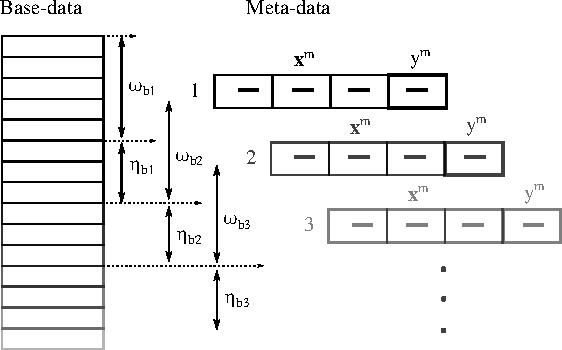
\includegraphics[width=0.5\linewidth]{ms_diag0_off}
    \caption{Extração de meta-atributos da janela $\omega_b$ e obtenção de
    rotulo da janela $\eta_b$.}
    \label{fig:ms_diag0_off}
\end{figure}

Em seguida, os modelos induzidos são avaliados nos exemplos da janela
$\eta_{b1}$, onde o algoritmo que produziu o modelo de melhor performance
preditiva é definido como rótulo de $y^m$. Esse processo gera o primeiro
meta-exemplo. O mesmo processo é aplicado continuamente por $N$ passos, onde
$N$ é o número mínimo de instâncias para induzir um modelo consistente para
gerar os meta-dados iniciais. Esses $N$ meta-exemplos serão os primeiros dados
que serão usados para induzir modelos na fase online.

\subsection{Fase Online}
\label{subsec:online}

Na fase online, o \textit{framework} recebendo um contínuo fluxo de dados.
Inicialmente, ele recebe um vetor de atributos $\boldsymbol{x}_b =
(x_1,...,x_p)$, e após algum atraso, o atributo rótulo $y_b \in \{0,1,..,k\}$
para classificação, onde $k$ é o número de classes ou $y_b \in \rm{I\!R}$ para
regressão.

A Figura \ref{fig:ms_diagram0} mostra um dado momento $t$ na fase online. Ele
tem uma janela de tamanho fixo $\omega_b$ que será usado para induzir um
modelo, uma janela de tamanho fixo $\eta_b$ onde o modelo induzido em
$\omega_b$ será avaliado assim que o rótulo referente for descoberto, um
tamanho $\gamma_b$ que é o atraso em observar o rótulo para os exemplos na
janela $\eta_b$ e uma janela de tamanho variável $\lambda_b$ de exemplos
aguardando serem processados.
Quando $\gamma_b$ tem o mesmo tamanho que $\eta_b$, isto é, todos os rótulos de
$\eta_b$ foram obtidos, a janela $\omega_b$ é deslizada $\eta_b$ instâncias
para a direita e um novo modelo é induzido nessa janela.

\begin{figure}[ht]
    \centering
    \includegraphics[width=0.5\linewidth]{metastream_diag0}
    \caption{Discretização de janelas no nível base do fluxo de dados.}
    \label{fig:ms_diagram0}
\end{figure}

MtA entra em ação no segundo nível de processamento, nomeado nível meta. Como
mostrado na Figura \ref{fig:ms_diagram1}, os meta-atributos são extraídos da
janela $\omega_b$ e geram o meta-exemplo sem o rótulo que é mantido para
atualização posterior.

\begin{figure}[ht]
    \centering
    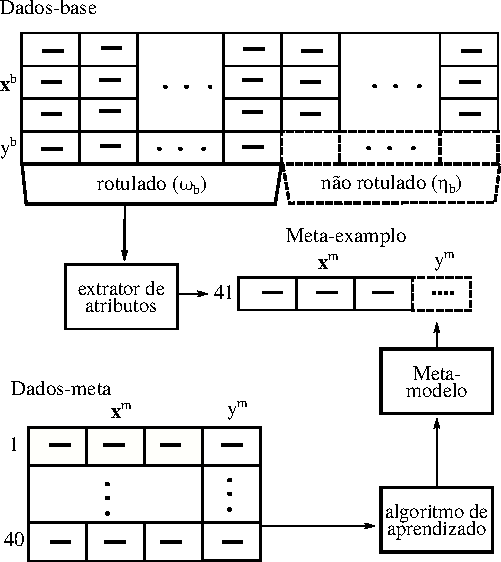
\includegraphics[width=0.5\linewidth]{metastream_diag1}
    \caption{Extração de meta-atributos das janelas  $\omega_b$ e $\eta_b$ no nível meta.}
    \label{fig:ms_diagram1}
\end{figure}

O algoritmo de aprendizado (meta-aprendiz) usa meta-exemplos rotulados
previamente na meta-base para induzir um meta-classificador, que é utilizado
para recomendar um algoritmo que induzirá um modelo usando a janela $\omega_b$
que provavelmente será o mais preciso para prever os rótulos dos exemplos em
$\eta_b$.



% Em \cite{goodfellow2016deep}, são listadas mas não limitadas à onze tarefas
% possíveis ao aprendizado supervisionado, para o problema proposto realizaremos
% duas dessas tarefas, a classificação e a classificação com valores faltantes.

% \subsection{Classificação}
% Esta tarefa $\boldsymbol{T}$ consiste em designar uma categoria para a entrada
% $\boldsymbol{x}$ dentro do conjunto finito $\mathcal K$ de $k$ categorias. Queremos
% então aproximar a função $f:\mathbb{R}^n\longrightarrow \{1,...,k\}$, tal que, dado
% um conjunto de entrada $\boldsymbol{x}$ a função designará um valor $y =
% f(\boldsymbol{x})$ onde $y \in \mathcal{K}$. Existem variantes desta tarefa, que
% não será abordada, onde ao invés de designar uma classe precisa à entrada
% $\boldsymbol{x}$, é dado um vetor de probabilidades sobre todas as classes de
% $\mathcal K$ \cite{goodfellow2016deep}.

% % FAZER UM DIAGRAMA SIMILAR AO LEARNING FROM DATA pagina 30

% \section{Fluxos de Dados e Mudança de Conceito}
% \label{sec:fluxos-de-dados-e-mudanca-de-conceito}
% Uma série temporal é um conjunto de observações obtidas sequencialmente no tempo
% \cite{box2015time,brockwell2016introduction,durbin2012time}, onde o eixo temporal
% costuma estar ligado a frequência em que esses dados são gerados, ex. meses, para
% as vendas mensais de uma loja ou mili-segundos, para as transações de ações na
% bolsa de valores. Sendo uma série temporal um processo estocástico indexado
% \cite{hamilton1994time}, esse pode apresentar dependências temporais devido seu
% processo gerador, eventos futuros são influenciados por eventos passados
% \cite{karlin2012first}. Neste trabalho iremos nos ater a formalização do modelo
% de \textit{espaço de estados} aditivo \cite{durbin2012time}.
% \begin{definition}
%     Uma série temporal é um conjunto de observações $S=\{x_1,...,x_n\}$ indexadas
%     por $n \in \mathbb{N}$.
% \end{definition}

% O aprendizado apresentado na seção \ref{sec:aprendizado-de-maquina} é do tipo
% indutivo, ele se baseia no axioma empiricista de que o futuro irá se comportar
% como o passado \cite{vickers2009problem}, estatisticamente, que os dados serão
% estacionários gerados de uma mesma função de probabilidade. Em ambientes
% complexos e com dependência temporal, essa premissa pode não ser verdadeira
% \cite{hulten2001mining}. Em fluxos de dados, que serão discutidos na seção
% \ref{sec:fluxo-de-dados}, é comum tal mudança, portanto é necessário desenhar
% sistemas capazes de se adaptar a essas condições \cite{gama2007learning}.

